\chapter{Fundamental Units and Laws of Electric Circuits}
\label{chap:fundamentals}
This chapter will introduce all of the foundational concepts of circuits. After you've read this chapter, almost everything else we cover will be derived from or otherwise based on these concepts. I'll recap all of these concepts more concisely at the end of the chapter so you can refer back to that section later in the course.

\section{The Basic Units of Circuits}
It's a real drag to have to start with units, but I think doing so will make everything else easier. As it turns out, there are only a handful of units that we will use during this course, and I want to introduce most of them now so you'll know what I'm talking about as we progress.
\par
The first and most foundational unit I want to introduce is the \textbf{Coulomb (C)}. The coulomb is the unit of charge, without which we would be living in a sad universe without electronics. Charge is carried through circuits by electrons. Electrons each have -1.602$\times10^{-19}$ coulombs of charge\footnote{Fun fact: as a result of the redefinition of the SI unit of current (the Ampere) in May 2019, the value of the electron charge $q_e$ has been numerically defined as \textit{exactly} $-1.602176634\times10^{-19}$ C. Impress all your friends with this knowledge. (See https://www.bipm.org/en/publications/si-brochure/ for more information on this exciting topic.)}, so when we mention coulombs, know that a single negative coulomb is carried by $6\times10^{18}$ electrons. That's nearly as many electrons as there are grains of sand on earth!\footnote{according to this estimate:
https://www.npr.org/sections/krulwich/2012/09/17/161096233/which-is-greater-the-number-of-sand-grains-on-earth-or-stars-in-the-sky
} But enough about charge. Charge only makes circuits work if it's \textit{moving}.
\par
\begin{figure}[h!]
\centering
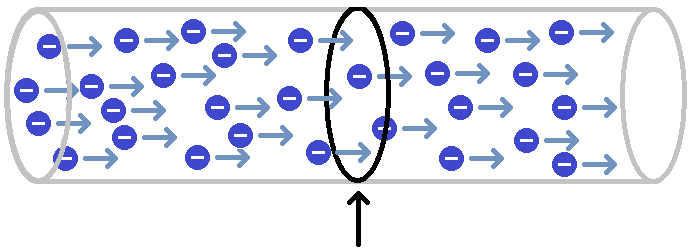
\includegraphics[width=10cm]{figures/electronFlow.png}
\caption{Electrons on-the-move! This is just an artistic rendition of what flowing charge in a wire looks like.}
\label{movingChargeThroughHoop}
\end{figure}
This brings us to the \textbf{Ampere (A)}. The ampere (or amp) is a unit that helps us describe how fast charge is moving, and its definition is 1A = 1C/1s. The diagram in Figure \ref{movingChargeThroughHoop}, which depicts electrons flowing through a section of wire, may help you visualize this. The electrons in this diagram are all flowing in the same direction, and the value of their resulting current is given by the total amount of charge that flows past a given point (denoted by the black arrow) in one second. Practically speaking, a 1A current is relatively large, especially in the context of consumer electronics like a smartphone or your computer. For historical reasons\footnote{Ben Franklin was involved, y'all.} conventional current flow is in the opposite direction of electron flow. This mostly has to do with the fact that the charge of an electron is negative, which wasn't realized until the standard for current flow was set. Don't fret, though---after this section, we will only talk about conventional current flow in this class. 
\par
Electrons must be moving to establish current, which means those electrons need kinetic energy. That kinetic energy is imparted to electrons by \textit{voltage} sources, which provide an electric potential energy difference in units of \textbf{Volts (V)}, where 1V=1J/1C. A voltage difference is to electrons like a hill is to a ball. If you put a ball up on a hill, it will start rolling down, gaining kinetic energy as its height decreases. Similarly, if you put an electron at a low voltage, it will drift toward a higher voltage. This low-to-high movement is caused by the fact that the electron's charge is negative. Don't get too hung up on the analogy; just remember that conventional current flows from the positive voltage to the negative voltage of a power supply. 
\par
In a circuit, any point at which multiple (two or more) elements are connected is referred to as a \textbf{node}, and every node has a single voltage. When we refer to voltage, we either do so in terms of voltage \textit{differences} between nodes, or we talk about a voltage in a circuit with respect to a reference node called the \textbf{ground} node.
\par
You have probably already seen power in at least one other course, but as I mentioned in the last chapter, it's a big reason why we have circuits at all. Power is the amount of energy that is supplied by a power source or \textit{dissipated} (i.e., used up) by a circuit element over time. Power is measured in \textbf{Watts (W)}, where 1W = 1J/1s. Using your dimensional analysis skills, you can confirm that power (P) is related to current (i) and voltage (V) by the following expression, known as \textit{Watt's Law}:
$$
P = i\times V
$$
\par
In words, this states that the power (in Watts) dissipated or supplied by an element is given by the current flowing through that element multiplied by the voltage across that element. 

\begin{figure}[h!]
\centering
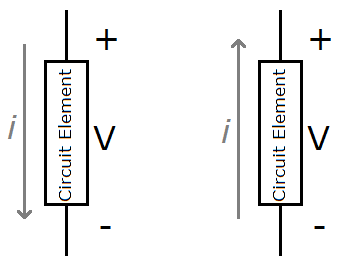
\includegraphics[width=10cm]{figures/powerSuppliedDissipated.png}
\caption{The element on the left side of this figure is dissipating power, because the current is flowing through the element from its higher voltage side to its lower voltage side. Conversely, the element on the right side of this figure is supplying power in the circuit, because the current is flowing through the element from its lower voltage side to its higher voltage side.}
\label{powerSuppliedDissipated}
\end{figure}

If the current is going in the direction of the voltage drop across the element---that is, into the terminal with greater voltage and out of the terminal with smaller voltage---then the element is dissipating that power. If the current flows in the opposite direction through the element, then that element is supplying power. Figure \ref{powerSuppliedDissipated} illustrates this convention. In either case, $V$ represents the voltage \textit{across} the source or element, and $i$ represents the current flowing \textit{through} the source or element.
\par
To facilitate the introduction of the last unit of this chapter, we need to look at a circuit. Figure \ref{resistorBatteryCircuit} shows the simplest circuit I could come up with to introduce \textit{resistance}.
\begin{figure}[h!]
\centering
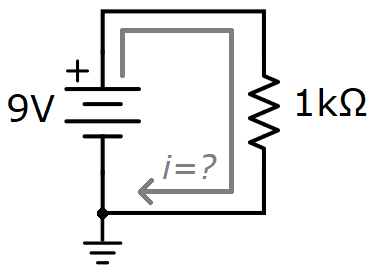
\includegraphics{figures/batteryResistorCircuit.png}
\caption{A simple circuit with a battery and a single resistor. The current in this circuit flows in the direction of the arrow.}
\label{resistorBatteryCircuit}
\end{figure}
Before we proceed, let's dissect this schematic a bit. In this circuit, there is a battery---represented by four horizontal lines and a plus sign---and a \textit{resistor}---the zig-zagged symbol on the right-hand side of the schematic. All of the straight lines that connect the elements in the circuit can be thought of as wire; these are the \textit{nodes} of the circuit. There is also a symbol at the bottom left of the circuit with three horizontal black lines that cross a vertical line connected to the bottom left node of the circuit. This symbol marks the ``ground'' node. It is common practice to include a circuit ground in schematics; ground is treated as the 0V reference for the circuit, which makes calculations and debugging easier. 
\par
The battery is labeled ``9V'', meaning there is a 9 volt \textit{difference} between its positive and negative (top and bottom) terminals. This also means there is a 9V difference between the nodes connected to its positive and negative terminals. 
\par
The gray arrow denotes the direction of current flow in this circuit---out of the positive terminal of the battery, through the resistor, and into the negative terminal of the battery. The value of the current is the same at all points along this loop.
\par
%Ohm's law
The resistor is labeled ``1k$\Omega$'', which is its resistance in \textbf{Ohms ($\Omega$)}. The \textbf{Ohm} is the unit of resistance (or impedance), and it relates the current flowing through an element to the voltage difference across that element. Initially, this unit was defined empirically upon the observation that voltage and current are approximately linearly proportional in most materials. Dimensionally, the Ohm is defined according to the following relationship:
$$
1\Omega = \frac{1V}{1A}
$$
\par
In order to determine the value of the current flowing in this circuit, we will need to use \textbf{Ohm's Law}:
$$
V=i \times R
$$
In words, this law states that the voltage difference across (or the voltage drop over) the resistor is equal to the value of the current flowing through the resistor (represented as $i$) multiplied by the resistance of the resistor ($R$). The voltage across the resistor is defined by the battery as 9V. Since we know the value of the resistance is 1000$\Omega$, we can rearrange Ohm's law to find the value of the current flowing through the resistor:
$$
i = \frac{9\textrm{V}}{1000\Omega} = 0.009 \textrm{A}
$$
Figure \ref{resistorBatteryCurrentCircuit} shows the fully-annotated schematic for this circuit.
\begin{figure}[h!]
\centering
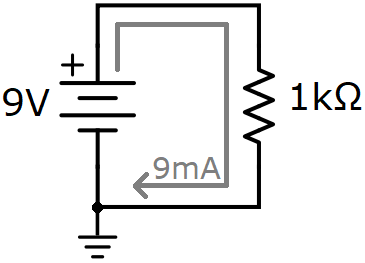
\includegraphics{figures/batteryResistorCurrentCircuit.png}
\caption{The circuit of Figure \ref{resistorBatteryCircuit}, with current labelled.}
\label{resistorBatteryCurrentCircuit}
\end{figure}
\par
To save time later, I will use the prefixes M ($10^6$), k ($10^3$), m ($10^{-3}$), $\mu$ ($10^{-6}$), n ($10^{-9}$), and p ($10^{-12}$)to represent orders of magnitude for the quantities we calculate. Current is usually on the order of $10^{-3}$A, or mA, and resistors are often on the order of $10^{3}\Omega$, or k$\Omega$. The nice thing about these unit prefixes is that they cancel each other out when multiplied: 1mA$\times$1k$\Omega$ = 1A$\times$1$\Omega\times\cancel{10^3\times10^{-3}}$ = 1V. They also often convert to one another in calculations through the property that $\frac{1}{m} \rightarrow k$ and $\frac{1}{k} \rightarrow m$. Using these prefixes, we cite the current in the circuit of Figure \ref{resistorBatteryCurrentCircuit} as 9mA. The other prefixes will come up later, too, but I will try to remind you of their meaning when they do.
\par
We've now seen all the fundamental units of circuits, but let's use Watt's law to fully characterize the behavior of the circuit in Figures \ref{resistorBatteryCircuit} and \ref{resistorBatteryCurrentCircuit}. Having found the value of the current in this circuit, we have almost completely defined its behavior. However, remember that all circuits either power devices or condition signals, and even though this circuit is mostly instructive in purpose, let's assume that the whole point of this circuit is to provide power to the resistor. If that's the case, we need to determine how much power the resistor is receiving. To do so, we will rely on Watt's Law. Looking again at our circuit in Figure \ref{resistorBatteryCurrentCircuit}, if the voltage across the resistor is 9V and the current through the resistor is 9mA, then the power dissipated by the resistor is $9\textrm{mA}\cdot9\textrm{V} = 81\textrm{mW}$. Likewise, since there are 9V across the battery terminals and the current flowing through the battery is 9mA, the battery is \textit{supplying} 81mW. It is always good to verify that the power supplied by the sources in a circuit is equal to the power dissipated by the elements of a circuit; this is a good way to double-check your calculations. Energy is always conserved, after all...even in circuits!
\par
Before moving on, let's use Ohm's law to generate two additional forms of Watt's Law. If we combine Ohm's law with Watt's law, we can derive the following alternate form for Watt's law:
$$
P = i\times V = i\times(i\times R) = i^2\times R
$$
Additionally, if we rearrange Ohm's law as i = $\frac{V}{R}$, then we can use this definition of current in Watt's law in the following way:
$$
P = i\times V = \frac{V}{R}\times V = \frac{V^2}{R}
$$

In analyzing circuits, you will sometimes find one of these forms of Watt's Law to be more useful than the others. You should be able to quickly recall all of these forms or at least derive them.
\subsection{More Schematic Symbols for Power Supplies}
The example circuit in Figure \ref{resistorBatteryCurrentCircuit} includes a battery, which is one type of DC power supply. There are two other symbols for DC supplies you should know about so that when they come up in future chapters you won't be lost. 
\begin{figure}[h!]
\centering
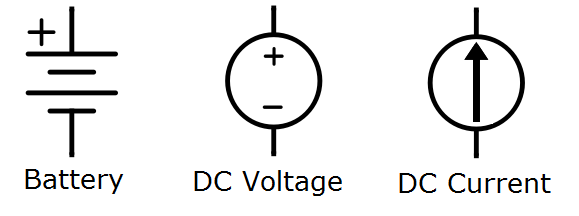
\includegraphics{figures/DCpowerSupplies.png}
\caption{Common DC power supply symbols.}
\label{DCpowerSupplies}
\end{figure}
\par
Figure \ref{DCpowerSupplies} shows all the types of DC power supplies you can expect to see in this course. (There are AC power supplies, too, but those will be introduced in Chapter \ref{chap:ACcircuits}.) The symbol on the far left of this figure represents a battery, which we have already seen. Batteries provide a constant voltage difference between their two terminals. The circular symbol in the middle of Figure \ref{DCpowerSupplies} with terminals marked ``+'' and ``-'' represents a DC voltage supply more generally; it could represent any regulated DC voltage supply or a battery. The circular symbol on the far right of the figure with an arrow running from one of its terminals to the other represents a DC current source. For powering electronics, voltage sources are superior to and far more prevalent than DC current sources. As a result, there are not many examples of DC current sources in your everyday life, with one notable exception---your phone charger. Like most battery chargers, a phone charger provides a steady current in reverse through the battery in order to put charge carriers back into the negative terminal of the battery. We will use current sources in calculations at times in this course, but they are more useful and practical in circuit analysis than in everyday use.

\section{(Additional) Fundamental Laws}
In the process of introducing the basic units of circuits in the previous section, I also introduced two of the most import laws of circuits---Ohm's and Watt's Laws. In this section, I will introduce the two remaining fundamental laws of circuits---Kirchhoff's Current Law and Kirchhoff's Voltage Law---by deriving them while we investigate the properties of two more circuits.
\begin{figure}[h!]
\centering
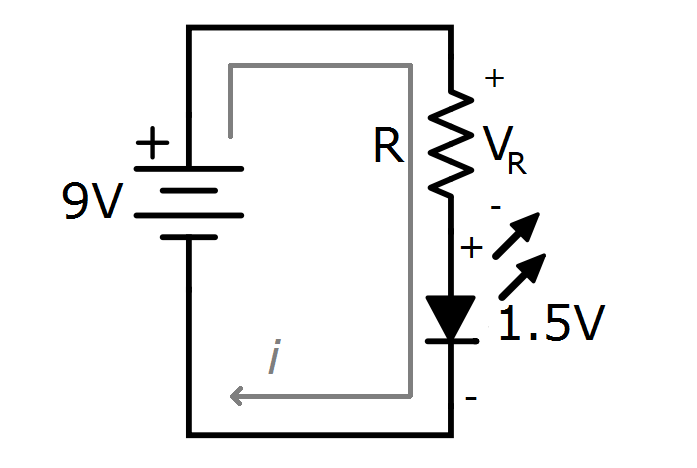
\includegraphics[width=10cm]{figures/LEDCircuit.png}
\caption{A circuit that lights up an LED.}
\label{simpleLED}
\end{figure}

The circuit of Figure \ref{simpleLED} is designed to light up (provide power to) a light-emitting diode (LED) without destroying it. There are only three elements in this circuit: a battery, a resistor, and an LED (whose symbol looks like a big arrow pointing directly at a line, with little floating arrows above and to the right of it). Let's assume that the LED can handle at most 30mW, and that we need to find a value for resistor ``R'' that will ensure this power limit is obeyed. The battery voltage is 9V, the resistor has a resistance of \textit{R}, and the LED, when operating, has a constant 1.5V across it\footnote{I'm not going to describe how LEDs physically work in this class, but when an LED is emitting light, we can assume there is some constant voltage across it. 1.5V is a realistic voltage, but different LEDs can have different voltage values depending on the color and fabrication parameters of the LED.}. The current, $i$, is shown in gray.  If I want to know how much power the LED is using, I just need to know the voltage across it and the current flowing through it. Then I can use Watt's Law to solve for the power being dissipated by the LED. For the circuit of Figure \ref{resistorBatteryCircuit}, I knew the voltage across the resistor and the resistance itself, and that information allowed me to use Ohm's law ($V=i \times R$) to find the current flowing through that circuit. In the circuit of Figure \ref{simpleLED} however, the voltage across the resistor is not given. To find it, we need to use \textbf{Kirchhoff's Voltage Law} (which I will refer to as \textbf{KVL} from now on):
$$
\textrm{Around any loop in a circuit,} \sum\textrm{\{voltage added\}} = \sum\textrm{\{voltage dropped\}}
$$
Or, in shorthand, 
$$
\sum_{loop}\Delta V^+ = \sum_{loop}\Delta V^- \textrm{  or simply }\sum_{loop}\Delta V = 0
$$
In words, this states that if I trace through a complete loop (starting and stopping at the same node) of a circuit, I will encounter voltage drops and voltage increases, and for any such loop, the amount of voltage dropped will be equal to the amount of voltage added. If I trace clockwise through the circuit of Figure \ref{simpleLED} starting at the bottom left corner, I encounter the 9V increase of the battery, then an unspecified voltage drop across the resistor, and then the 1.5V drop across the LED, which takes me back to the node where I started. The increases in voltage and the voltage drops in that loop should sum to zero. Writing this out as an equation,
$$
9\textrm{V} - V_R - 1.5\textrm{V} = 0
$$
From this equation we see that the voltage drop across the resistor, $V_R = 7.5\textrm{V}$.
\par
With the voltage across the resistor determined, we can solve for the current flowing through the resistor and the LED in terms of the resistance, $R$. Remember that the purpose of this circuit is to provide power to the LED \textit{without destroying it}, and that the LED can handle \textit{at most} 30mW. If that's the case, then according to Watt's Law, the following expression must be true:
$$
1.5V \cdot i \leq 30\textrm{mW}
$$
To enforce this requirement, we must set $R$ so that the current does not exceed 30mW/1.5V, or 20mA. Using this expression for current and the fact that $V_R=7.5\textrm{V}$ along with Ohm's law, we can set a \textit{lower-bound} (R$_{min}$) on the range of allowable values for $R$ in the following way:
$$
7.5\textrm{V} = i \times R_{min} = 20\textrm{mA} \cdot R_{min},
$$
therefore
$$
R_{min} = \frac{7.5\textrm{V}}{20\textrm{mA}} = 375\Omega
$$
\par
So, in order for the LED in Figure \ref{simpleLED} to light up and not \textit{burn} up, the resistor value must be \textit{at least} 375$\Omega$. If you followed along with this example, congratulations! You just experienced a taste of electric circuit design!
\par
%KCL
There is one last fundamental law to introduce, and to do so we will look at the circuit of Figure \ref{twoLEDs}.
\begin{figure}[h!]
\centering
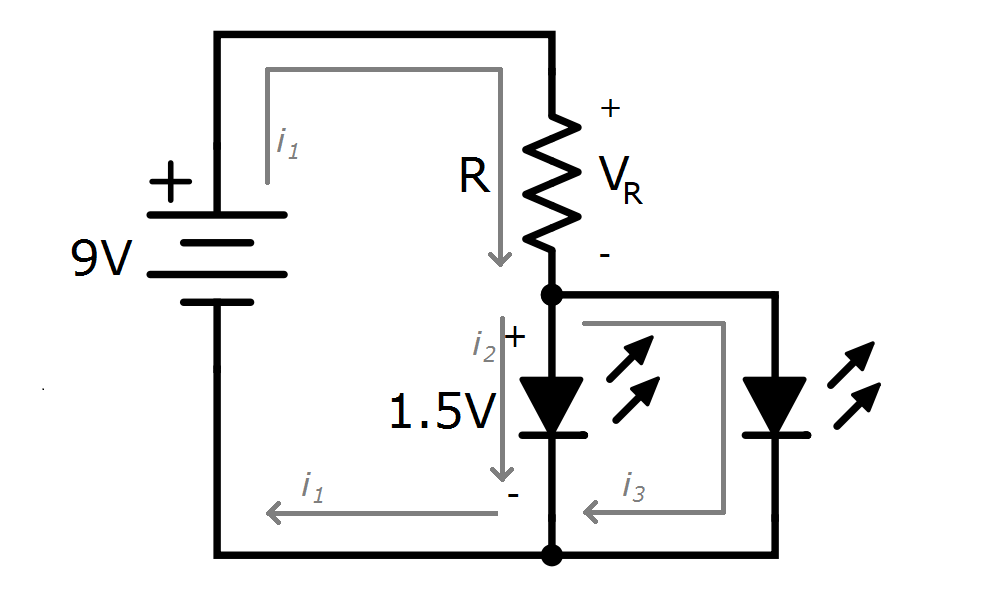
\includegraphics[width=12cm]{figures/twoLEDsCircuit.png}
\caption{A circuit that lights up two LEDs.}
\label{twoLEDs}
\end{figure}

This circuit is comprised of a battery, a resistor, and two LEDs. As before, the voltage across both of the LEDs is 1.5V, and KVL tells us that the voltage across the resistor must be 7.5V. However, this circuit has more than just one full loop. The dot connecting the resistor and the two LEDs indicates that all three wires converging there form a node. At that node, current $i_1$ enters from the resistor branch and currents $i_2$ and $i_3$ exit through the two LED branches. We can relate these three currents usign \textbf{Kirchhoff's Current Law} (which I will refer to as \textbf{KCL} from now on): 
$$
\textrm{At any node in a circuit,} \sum\textrm{\{current entering\}} = \sum\textrm{\{current leaving\}}
$$
Or, in shorthand
$$
\sum_{node}i_{in} = \sum_{node}i_{out}
$$

In words, this means that the amount of current flowing into a node must be equal the amount of current flowing out of that node. In our circuit, this means that $i_1=i_2+i_3$. Let's assume that both LEDs are identical, and therefore the current flowing through each LED is the same. In that case, $i_2=i_3$. Let's also assume that we need to enforce the same constraints on the power delivered to each LED as before---$P_{LED}\leq30\textrm{mW}$. Therefore, the current flowing through each LED must be constrained to be 20mA or less (we'll define $i_{2,max}=20\textrm{mA}$ and $i_{3,max}=20\textrm{mA}$). If we assume that each of these currents is at its maximum value, then $i_2=i_3=20\textrm{mA}$ and according to KCL, the maximum value for the current flowing through the resistor in this circuit $i_{1,max}=i_{2,max}+i_{3,max}=40\textrm{mA}$. As was the case in our analysis of the circuit in Figure \ref{simpleLED}, this maximum current value places a constraint on the possible resistance values of our resistor; given the fact that the voltage across the resistor is set at 7.5V, according to Ohm's Law, $R_{min}=7.5V/i_{1,max}=187.5\Omega$. This is half of the minimum resistance value we found for the circuit of Figure \ref{simpleLED}; why do you think that is?
\section{Recap: The Fundamentals}
In the previous section, I introduced several fundamental concepts without dwelling too much on definitions. I want to ennumerate and concisely define each of these concepts here again:
\begin{description}
\item[Charge] is measured in \textit{Coulombs} (C) and is the foundational measure of electronics. An electron has a charge of -1.602$\times10^{-19}$C, which means that a single negative coulomb is made up of LOTS of electrons.

\item[Current] is measured in \textit{Amperes} (A) (or just \textit{Amps}) and is defined as the flow of charge through an element or elements. Dimensionally, 1A=1C/1s. Current that flows through a single branch has a constant value at all points along that branch.

\item[Nodes] are points in a circuit at which multiple (two or more) elements are connected. Each node has a constant voltage.
\item[Ground] is the node in a circuit with respect to which all other node voltages are referenced; if a specific voltage value is cited at a point in a circuit, that is usually relative to ground.

\item[Voltage] is measured in \textit{Volts} and is defined as energy per unit charge. Dimensionally, 1V=1J/1C. We often refer to voltage \textit{across} an element; by this, we mean the \textit{difference} between the voltages at the two ends of that element. We also sometimes refer to voltage at a node with respect to the voltage at another node, usually the \textit{ground} node.

\item[Power] is measured in \textit{Watts}, and is defined as energy supplied or dissipated over time. Dimensionally, 1W=1V$\cdot$1A.\footnote{1W=1J/1s of course, but the definition above is generally more useful for this course. The standard definition can be derived from 1W=1V$\cdot$1A without too much effort.} Power in circuits is typically supplied by voltage or current sources and dissipated by resistors.

\item[Watt's Law] is the name for the law that relates power supplied or dissipated by a circuit element to the current flowing through that element and the voltage across that element. Through the use of Ohm's Law, several forms of Watt's Law can be derived: 
$$
P = i \times V = i^2 \times R = \frac{V^2}{R}
$$

\item[Resistance] is measured in \textit{Ohms}, and it relates the voltage across a resistor to the current flowing through that resistor. Dimensionally, $1\Omega$=1V/1A. Resistance is the real (as opposed to imaginary) part of a broader relationship between current and voltage known as \textit{impedance}, which we will introduce later in the course.

\item[Ohm's Law] is related to resistance, and it states that the value of the voltage across a resistive element is equal to the value of the current flowing through that element multiplied by the resistance of that element:
$$V=i \times R$$

\item[Kirchhoff's Voltage Law (KVL)] states that around any loop in a circuit, the voltage added is equal to the voltage dropped:
$$\sum_{loop}{\Delta V^+} = \sum_{loop}{\Delta V^-}$$
This law is an expression of the concept of conservation of energy; all the energy delivered to a circuit must be dissipated by that circuit.
\item[Kirchhoff's Current Law(KCL)] states that at any node in a circuit, the current flowing in is equal to the current flowing out:
$$\sum_{node}{i_{in}} = \sum_{node}{i_{out}}$$
This law is an expression of the concept of conservation of mass; however many electrons flow into a node must also flow out of that node.
\end{description}
\par
These concepts may seem overwhelming all at once, but everything we do now will rely on these. If you read this whole chapter, you have now seen \textit{every} fundamental concept pertaining to electric circuits.